\chapter{Randomness} \label{ch:pbbasics}

This chapter introduces the basic concepts, axioms and theorems in probability theory.

\section{Randomness and Stochasticity}

People use \mync{random} and \mync{stochastic} to describe a variable or a model whose measurements or outcomes are not precisely predictable.

By saying \mync{randomness}, we often refer to the case where a variable (as in ``random variable'') is not predictable. Its value is not known precisely until it is measured. The chance of it taking particular values may follow some patterns known as the statistic property of the variable. For example, the result of tossing a coin is a random variable with the following statistic property. It is either head ($X=1$) or tail ($X=0$), each with a $50\%$ chance. The precise value remains unknown until the coin is tossed.

By saying \mync{stochasticity}, we often refer to the case where the outcome of a process (as in ``stochastic process'') is not predictable. This is likely caused by the incomplete modeling or random disturbance of the system. As a result, the process becomes non-deterministic, i.e., the output of the system cannot be precisely determined by the model and the input. A stochastic process can still be described by a parametric model, but with some unknowns (usually in the form of random variables) in the equations.

This part of the notebook mainly studies random variables. Stochastic process and control of stochastic systems are introduced elsewhere in control system related notebooks.

\subsection{Random Experiment}

``Experiment'' is one of the most important activities in science and engineering. Very often, experiments are used to verify a theory. In these cases, experiments are carefully designed so that its outcome is deterministic and predictable as long as the theory is correct. By observing the results of the experiments matching the prediction of the theory, we build confidence in the theory.

However, this notebook concerns with another type of experiments where the result of an experiment contains randomness due to the lack of information or incomplete modeling. Such experiments include tossing a coin, predicting the GDP of a country next year, etc. These experiments are known as \mync{random experiments}. The result of a random experiment can still be meaningful because it reflects some insights of the system. The challenge is to design the experiments so that useful information can be revealed from the result efficiently.

\subsection{Sample Space}

A set $S$ that consists of all possible outcomes of a random experiment is called a \mync{sample space}.

\mync{Cardinality} refers to the number of elements in a set. Depending on the cardinality of a sample space, it can be categorized as follows. If a sample space has a finite number of elements, it is called a \mync{finite sample space}. Otherwise, it is called an \mync{infinite sample space}. If the elements in an infinite sample space can be mapped to natural numbers, the sample space is also called a \mync{countably infinite sample space}. Otherwise, the sample space is called a \mync{uncountably infinite sample space}. Examples are given below.
\begin{itemize}
	\item Finite sample space. Randomly pick 5 balls out of a bag that contains 50 red balls and 50 green balls. The number of red balls in the picked 5 balls forms a finite sample space, $S = \{0, 1, 2, 3, 4, 5\}$.
	\item Countably infinite sample space. The number of continuous ``heads'' when tossing a coin before the first ``tail'' forms a countably infinite sample space, $S = \mathbb{N}$.
	\item Uncountably infinite sample space. Randomly drop a ball into a circle with radius of $1$. The distance of the ball to the center of the circle, $S=[0,1]$.
\end{itemize}

\begin{mdframed}
\noindent \textbf{Countable Infinity VS Uncountable Infinity}

Though both infinity, the total number of natural numbers, i.e., the cardinality of $\mathbb{N}$, is less than the total number of real numbers, i.e., the cardinality of $\mathbb{R}$.

The cardinality of $\mathbb{N}$ is known as $\aleph_0$. It is also the cardinality of all rational numbers. In computing, it is also the cardinality of all computable numbers (i.e., numbers that can be computed to any desired precision by a finite terminating algorithm) and computable functions (i.e., algorithms). The total number of real numbers is known as $\aleph_1$. It is also the cardinality of all irrational numbers and complex numbers, the number of points on a line or in a high dimensional space $\mathbb{R}^n$ where $n$ is a finite integer.

Larger infinity quantities such as $\aleph_2, \aleph_3, \ldots$ are also defined, though they may not have an intuitive explanation as $\aleph_0$ and $\aleph_1$.

Deeper discussion of this topic requires advanced set theory and is not given in this notebook.
\end{mdframed}

Finite sample space and countably infinite sample space are also known as \mync{discrete sample space}, whereas non-countably infinite sample space, \mync{non-discrete sample space}.

\subsection{Event}

An \mync{event} is defined as a subset $A \subseteq S$, i.e., it is a portion of all possible outcomes. An event may or may not occur depending on the outcome of the experiment. In the special case where $A$ has only one element, the event is also called an \mync{elementary event}, or a \mync{sample}. Notice that all elementary events are mutually exclusive as each of them contains an independent outcome of the experiment. In the special case where $A=S$, the event is also called a \mync{certain event}.

\section{Probability}

Given an experiment and an event, it is unsure whether the event will occur, and \mync{probability} is a measurement of the likelihood that the event is going to occur. For example, if the probability is $50\%$, it means that the event has an equal chance of happening or not happening.

There are different ways to calculate the probability of events. A rigorous mathematical definition of probability, known as axiomatic approach, is introduced in Section \ref{subsec:probability_axioms}. But before that, classical approach, empirical approach and geometric probability are introduced. One may get confused with which is the ``true'' definition of probability. As will be shown later, though defined from different angles, they all point to essentially the same concept.

\subsection{Classical and Empirical Probabilities}

In the \mync{classical approach}, it is assumed that all elementary events have the same chance of occurrence, and the total number of the elementary events is a finite and known number, $n$. Define an event that contains $h$ elementary events. The \mync{classical probability} of the event is given by $h/p$.

Calculating the cardinality of event $A$ and sample space $S$ is the key to solving the classical probability. Permutation and combination are widely used for such calculations. Suppose that there are $n$ distinct objects, and we would like to select $r\leq n$ objects from them and put them into a sequence. The \mync{permutation} defined by
\begin{eqnarray}
  nPr &=& n(n-1)(n-2)\cdots (n-r+1) \label{eq:permutation}
\end{eqnarray}
gives the number of possible outcomes. In the special case where $r=n$,
\begin{eqnarray}
  nPn &=& n(n-1)(n-2)\cdots \times 1 \nonumber
\end{eqnarray}
where $n(n-1)(n-2)\cdots \times 1$ is often denoted by $n!$. We can use that notation to rewrite \eqref{eq:permutation} as
\begin{eqnarray}
  nPr &=& \dfrac{n!}{(n-r)!} \nonumber
\end{eqnarray}
In permutation, the order of the selected $r$ objects matters. When the order does not matter, the \mync{combination} defined by
\begin{eqnarray}
  nCr &=& \dfrac{nPr}{r!} \nonumber \\
  &=& \dfrac{n!}{r!(n-r)!} \nonumber
\end{eqnarray}
is used to calculate the total number of outcomes. Notice that $nCr$ is also denoted by $\left(\begin{array}{c}
                                                                                           n \\
                                                                                           r
                                                                                         \end{array}\right)$.

In the \mync{frequency approach}, we can repeat the experiment $n$ times where $n$ is a large number, and record the number of instants where the event happened as $h$. The \mync{empirical probability} of the event is obtained by calculating $h/n$ which should converge to the true probability as $n$ grows.

\subsection{Geometric Probability}

\mync{Geometric probability} is an extension of the classical probability to infinite sample space. Similar with classical probability, it assumes that all elementary events share the same probability. The probability of an event can be obtained by measuring the area or volume associated with the event. An example is used to illustrate the use of geometric probability.

\begin{shortbox}
\Boxhead{Geometric Probability Example}
Consider two people trying to meet up at the park, but they forgot to tell each other the time to meet. Both of them will arrive at the park at anytime between $8:00$ AM and $9:00$ AM with equal chance, and wait for the other for 15 minutes or until $9:00$ AM, whichever is earlier, and then will leave the park if the other person does not show up.

Calculate the probability of the two people successfully meeting up.

\end{shortbox}

Since there are infinite number of combinations of the timestamps the two people arrive, we cannot calculate the total number of the sample space, nor the cardinality of the event of them successfully meeting up. Both of them are infinite sets. To solve the problem, consider drawing the sample space in a 2-D plot as shown in Fig. \ref{fig:geometricprobexp}, where the x-axis and y-axis are the arriving time of the two people, respectively. The shaded area represents the samples where the two would meet up successfully.

Divide the shared area by the total sample space area to get $P=7/16=43.75\%$ which is the probability that the two would meet up successfully.

\begin{figure}[!htb]
	\centering
	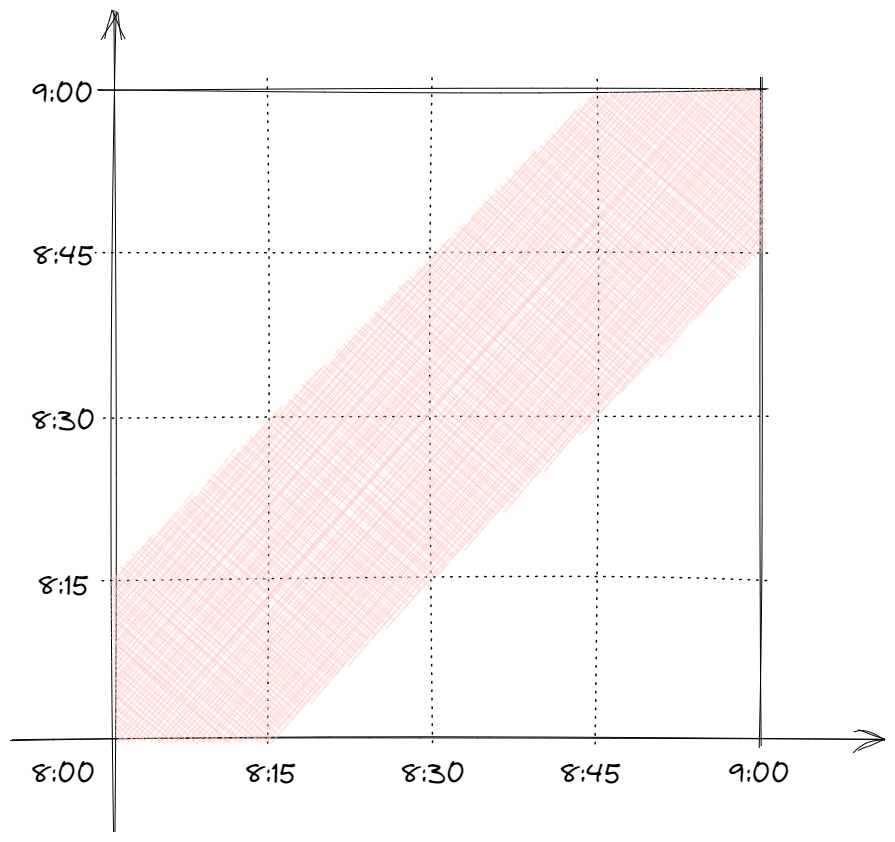
\includegraphics[width=0.5\textwidth]{chapters/part-1/figures/geometricprobexp.png}
	\caption{Sample space of two people arriving at part from 8:00 AM to 9:00 AM.} \label{fig:geometricprobexp}
\end{figure}

Note that in the problem description, the two people arrive at the part between $8:00$ AM and $9:00$ AM with equal chance. Here ``equal chance'' is an important prerequisite to use geometric probability. Otherwise, the probability of the event would have not been proportional to the area given in Fig.~\ref{fig:geometricprobexp}. This applies to most use cases of geometric probability.

\subsection{Axioms} \label{subsec:probability_axioms}

The \mync{axiomatic approach} puts things into mathematical prospective. 

Let the sample space be denoted by $S$, and events by $A_i$. For simplicity of illustration, assume that $S$ is discrete. Define $P(\cdot)$ as the \mync{probability function} and $P(A_i)$ the probability of the event $A_i$, subject to the following axioms:
\begin{enumerate}
  \item For every event $A_i$, $P(A_i)\geq 0$.
  \item For the certain event $S$, $P(S)=1$.
  \item For mutually exclusive events $A_1$ and $A_2$, $P\left(A_1\cup A_2\right) = P(A_1)+P(A_2)$.
\end{enumerate}

Using the above axioms, a bunch of well-known theorems can be derived, such as
\begin{itemize}
  \item If $A_1 \subseteq A_2$, $P(A_2-A_1) = P(A_2)-P(A_1)$.
  \item For every event $A_i$, $0\leq P(A_i) \leq 1$.
  \item For the impossible event $\varnothing$, $P(\varnothing)=0$.
  \item For the complement of an event $A\textprime$, $P(A\textprime)=1-P(A)$.
  \item For mutually exclusive events $A_i, i=1,...,n$, if $A = \bigcup_{i=1}^{n} A_i$, $P(A) = \sum_{i=1}^{n}P(A_i)$.
  \item For two events $A_1$ and $A_2$, $P\left(A_1\cup A_2\right) = P(A_1)+P(A_2)-P\left(A_1\cap A_2\right)$.
\end{itemize}

With the above axioms, we can revisit classical probability as follows. Assume that a discrete and finite sample space $S$ consists of the following elementary events $A_i, i=1,...,n$, i.e.,
\begin{eqnarray}
  S &=& \bigcup_{i=1}^{n} A_i \nonumber
\end{eqnarray}
and assume equal probabilities for all the elementary events, i.e., the probability of each event is given by
\begin{eqnarray}
  P(A_i) &=& \dfrac{1}{n}, i=1,...,n \nonumber
\end{eqnarray}
Define an event $A$ that is made up of $h$ such elementary events out of $A_i$. The probability of $A$ can then be calculated by
\begin{eqnarray}
  P(A) &=& \dfrac{h}{n} \nonumber
\end{eqnarray}
where $h$, $n$ are the cardinality of $A$ and $S$ with respect to the elementary events.

Recall the definition of a certain event. A certain event must have a probability of $1$. However, an event with probability $1$ is not necessarily a certain event. For example, consider dropping a ball in a circle. The probability of it landing precisely in the center of the circle is $0$ (yet possible), and the probability of otherwise is $1$ (yet not certain).

\begin{mdframed}
\noindent \textbf{Axiomatic approach Versus Frequency Approach}

Our intuitive understanding of probability should align with the frequency approach, where the probability of an event should describe how frequently an event occurs if the experiment is repeated many times. The axiomatic approach, though very clearly defined mathematically, seems to disconnect from the intuition.

As will be introduced in a later Section \ref{subsec:largenumbers}, the law of large numbers actually bridges the axiomatic approach and frequency approach, and guarantees the consistency of the two. As a result, the probability defined in axiomatic approach can also reflect the likelihood of an event happening the similar way the frequency approach does, and there is no gap in between.

\end{mdframed}

\subsection{Conditional Probability}

Assume two events $A$ and $B$. The \mync{conditional probability} $P(B|A)$ describes the probability of $B$ given that $A$ has occurred. The definition is given below. Think of this definition as $S$ replaced by $A$ since $A$ is confirmed occurred.
\begin{eqnarray}
  P(B|A) &\equiv& \frac{P(A\cap B)}{P(A)} \nonumber
\end{eqnarray}
Or equivalently,
\begin{eqnarray}
  P(A\cap B) &=& P(A)P(B|A) \nonumber
\end{eqnarray}
From the above,
\begin{eqnarray}
  P(B|A) &=& \dfrac{P(B)P(A|B)}{P(A)} \nonumber
\end{eqnarray}
which is known as the \mync{Bayes' rule}.

An example of implementing Bayes' rule is given below.

\begin{shortbox}
\Boxhead{Example of Bayes' Rule}

A couple has an equal chance of giving birth to a boy or a girl. Gather a group of couples with 2 children. Randomly pick one couple.

\begin{enumerate}
	\item Without further information, what is the chance of them having two girls?
	\item From an earlier interview, we know that they have at least one girl. What is the chance of them having two girls?
	\item From an earlier interview, we know that their first child is a girl. What is the chance of their second child being a girl as well?
\end{enumerate}

\end{shortbox}

In this example, the total sample space of a couple is 
\begin{eqnarray}
S &=& \left\{\left[\textup{Boy Boy}\right], \left[\textup{Boy Girl}\right], \left[\textup{Girl Boy}\right], \left[\textup{Girl Girl}\right]\right\} \label{eq:probsetexp}
\end{eqnarray}
each with a equal chance of $25\%$. For the convenience of illustration, define the following events.
\begin{itemize}
	\item Event $A$: both children are girls
	\item Event $B$: at least one child is a girl
	\item Event $C$: the first child is a girl
	\item Event $D$: the second child is a girl
\end{itemize}

Intuitively, we can see that the events are correlated in the following manner.
\begin{eqnarray}
	A &=& C \cap D \nonumber \\
	A, C, D &\subset& B \nonumber
\end{eqnarray}

Consider the first question. From \eqref{eq:probsetexp}, the chances of the event $A$ happening is obviously
\begin{eqnarray}
P(A) &=& \dfrac{1}{4} \nonumber
\end{eqnarray}
which is the answer to the first question.

Consider the second question. Using Bayes' rule,
\begin{eqnarray}
P(A|B) &=& \dfrac{P\left(A \cap B\right)}{P(B)} \nonumber \\
&=& \dfrac{P(A)}{P(B)} \nonumber \\
&=& \dfrac{1}{3} \nonumber
\end{eqnarray}
where notice that $P\left(A \cap B\right) = P(A)$ as $A\subset B$. Intuitively, this makes sense. From the interview, we are able to drop $\left[\textup{Boy Boy}\right]$ from the probable space for this couple. As a result, the chance of them having two girls, $\dfrac{1}{3}$, is higher than the case of the first question, $\dfrac{1}{4}$, where no priori information were available. In this example, the priori information is useful with getting a more precise answer.

Consider the third question. Using Bayes' rule,
\begin{eqnarray}
P(D|C) &=& \dfrac{P\left(D \cap C\right)}{P(C)} \nonumber \\
&=& \dfrac{P(A)}{P(C)} \nonumber \\
&=& \dfrac{1}{2} \nonumber
\end{eqnarray}
Notice that from \eqref{eq:probsetexp}, $P(D) = \dfrac{1}{2}$. Therefore, $P(D|C) = P(D)$. In this example, the prior information whether $C$ happens is not helpful with calculating the chance that $D$ happens. This makes sense. The gender of both children are independent. The fist child, either being a boy or a girl, does not affect the likelihood of the gender of the second child.

If $P(B|A)=P(B)$, or equivalently $P(A\cap B) = P(A)P(B)$, the two events $A$ and $B$ are known as \mync{independent events}. In this case, the priori knowledge of whether $A$ has occurred or not does not affect the probability of event $B$, and vice versa.
